\documentclass[border=2mm]{standalone}
\usepackage{tikz}
\begin{document}

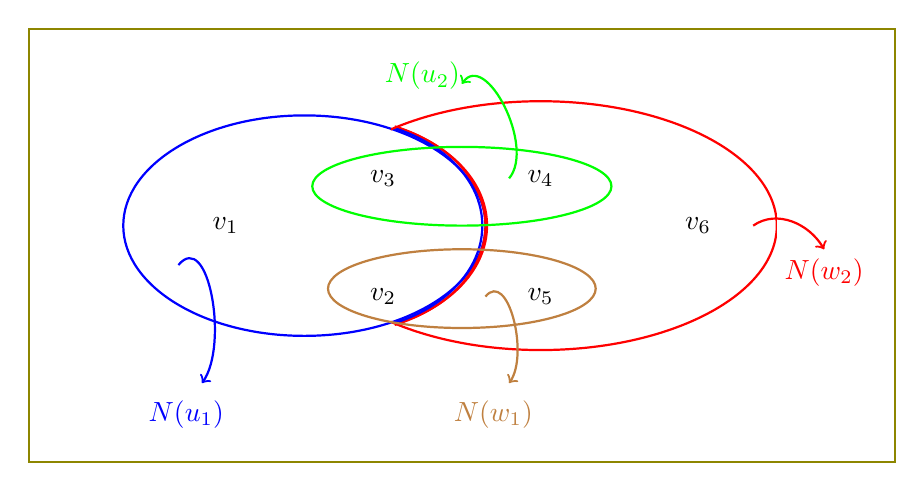
\begin{tikzpicture}[thick,
	set/.style = { circle, minimum size = .061cm}]
	
	% Background bounding box
	\draw [olive] (-2.5,-3) rectangle (8.5,2.5);
	
	% Large enclosing sets (drawn early for proper layering)
	\draw[blue] (1,0) ellipse (2.3cm and 1.4cm);
	
	% Red sets (clipped to right half-plane)
	\begin{scope}[red]
		\clip(2.15,-2) rectangle (7,2);
		\draw (1.4,0) circle [x radius=1.9cm, y radius=1.37cm];
		\draw (1.4,0) circle [x radius=1.92cm, y radius=1.36cm];
	\end{scope}
	
	\begin{scope}[blue]
		\clip(2.15,-2) rectangle (7,2);
		\draw (1.4,0) circle [x radius=1.86cm, y radius=1.35cm];
	\end{scope}
	
	\begin{scope}[red]
		\clip(2.1,-1.7) rectangle (7,2);
		\draw (4,0) circle [x radius=3cm, y radius=15.8mm];
	\end{scope}
	
	% Nested subsets (green and brown ellipses)
	\draw[green] (3,0.5) ellipse (1.9cm and 0.5cm);
	\draw[brown] (3,-0.8) ellipse (1.7cm and 0.5cm);
	
	% Vertex labels
	\node[black] at (0,0) {$v_1$};
	\node[black] at (2,0.6) {$v_3$};
	\node[black] at (2,-.9) {$v_2$};
	\node[black] at (4,0.6) {$v_4$};
	\node[black] at (4,-0.9) {$v_5$};
	\node[black] at (6,0) {$v_6$};
	
	% Annotation arrows and neighborhood labels
	\draw[->, blue] (-.6,-.5) to [out=50,in=55] (-.3,-2);
	\node[blue] at (-.5,-2.4) {$N(u_1)$};
	
	\draw[->, green] (3.6,0.6) to [out=50,in=55] (3,1.8);
	\node[green] at (2.5,1.9) {$N(u_2)$};
	
	\draw[->, brown] (3.3,-0.9) to [out=50,in=55] (3.6,-2);
	\node[brown] at (3.4,-2.4) {$N(w_1)$};
	
	\draw[->, red] (6.7,0) to [out=35,in=120] (7.6,-0.3);
	\node[red] at (7.6,-0.6) {$N(w_2)$};
	
\end{tikzpicture}

\end{document}
